%!TEX root = thesis.tex

\newpage

\makeatletter
\renewcommand\appendixname{Приложение}
\gdef\appendix{\par
\setcounter{section}{0}%
\setcounter{subsection}{0}%
\def\thesection{\@Alph\c@section}
\def\section##1{\refstepcounter{section}
\setcounter{table}{0}
\def\thetable{\@Alph\c@section.\arabic{table}}
\goodbreak\noindent{\indent\Large\bf\hbox to 8.5em{\appendixname\
\thesection\hss}\hspace{0.8ex}##1}%
\nobreak\vspace{1em}\nobreak\noindent%

\addcontentsline{toc}{chapter}{\hbox to 8.5em{\appendixname\ \thesection\hss}\hspace{0.8ex}##1}}}
\makeatother

\appendix

\section{ Исходные данные}
\label{c:source_data}
% latex table generated in R 3.1.2 by xtable 1.7-4 package
% Tue Mar  3 10:11:27 2015
\begin{table}[H]
\centering
\begin{tabular}{rrr}
  \hline
 & year & temperature \\ 
  \hline
1 & 1975.00 & 20.20 \\ 
  2 & 1976.00 & 16.00 \\ 
  3 & 1977.00 & 17.70 \\ 
  4 & 1978.00 & 16.75 \\ 
  5 & 1979.00 & 17.50 \\ 
  6 & 1980.00 & 16.77 \\ 
  7 & 1981.00 & 19.80 \\ 
  8 & 1982.00 & 19.00 \\ 
  9 & 1983.00 & 21.40 \\ 
  10 & 1984.00 & 19.40 \\ 
  11 & 1985.00 & 20.40 \\ 
  12 & 1986.00 & 16.50 \\ 
  13 & 1987.00 & 17.10 \\ 
  14 & 1988.00 & 23.80 \\ 
  15 & 1989.00 & 19.90 \\ 
  16 & 1990.00 & 18.50 \\ 
  17 & 1991.00 & 23.00 \\ 
  18 & 1992.00 & 21.90 \\ 
  19 & 1993.00 & 18.00 \\ 
  20 & 1994.00 & 21.40 \\ 
  21 & 1995.00 & 18.90 \\ 
  22 & 1996.00 & 19.10 \\ 
  23 & 1997.00 & 21.00 \\ 
  24 & 1998.00 & 18.40 \\ 
  25 & 1999.00 & 23.50 \\ 
  26 & 2000.00 & 21.00 \\ 
  27 & 2001.00 & 24.20 \\ 
  28 & 2002.00 & 23.10 \\ 
  29 & 2003.00 & 18.00 \\ 
  30 & 2004.00 & 19.10 \\ 
  31 & 2005.00 & 20.00 \\ 
  32 & 2006.00 & 21.30 \\ 
  33 & 2007.00 & 19.40 \\ 
  34 & 2008.00 & 21.80 \\ 
  35 & 2009.00 & 21.90 \\ 
  36 & 2010.00 & 24.30 \\ 
  37 & 2011.00 & 22.80 \\ 
  38 & 2012.00 & 20.20 \\ 
   \hline
\end{tabular}
\caption{Исходные данные.} 
\label{table:source}
\end{table}


\newpage
\section{ Графические материалы}
\label{c:graphs}

\setcounter{figure}{0}

\begin{figure}[H]
	\center{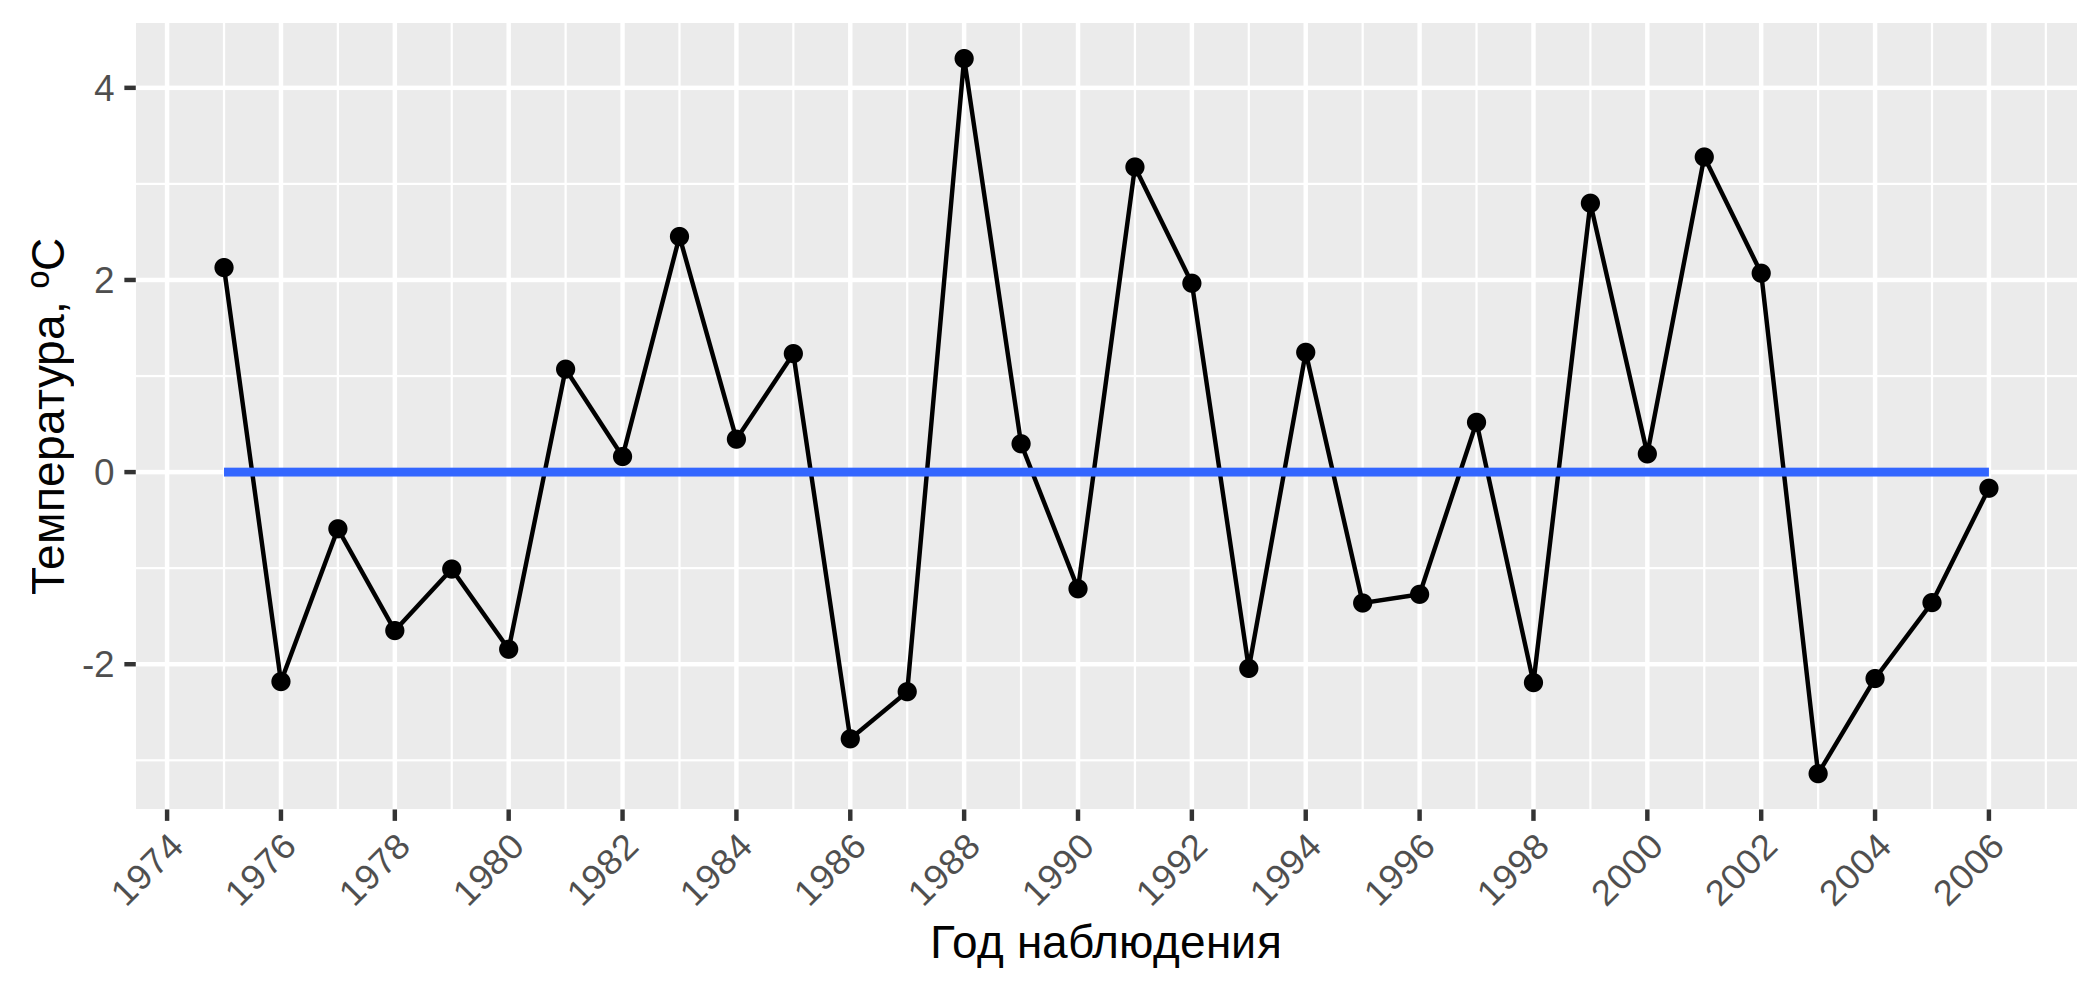
\includegraphics[width=1\linewidth]{../figures/residual/time-series.png}}
\caption{График ряда остатков}
\label{img:ts_detrended}
\end{figure}

\begin{figure}[H]
	\center{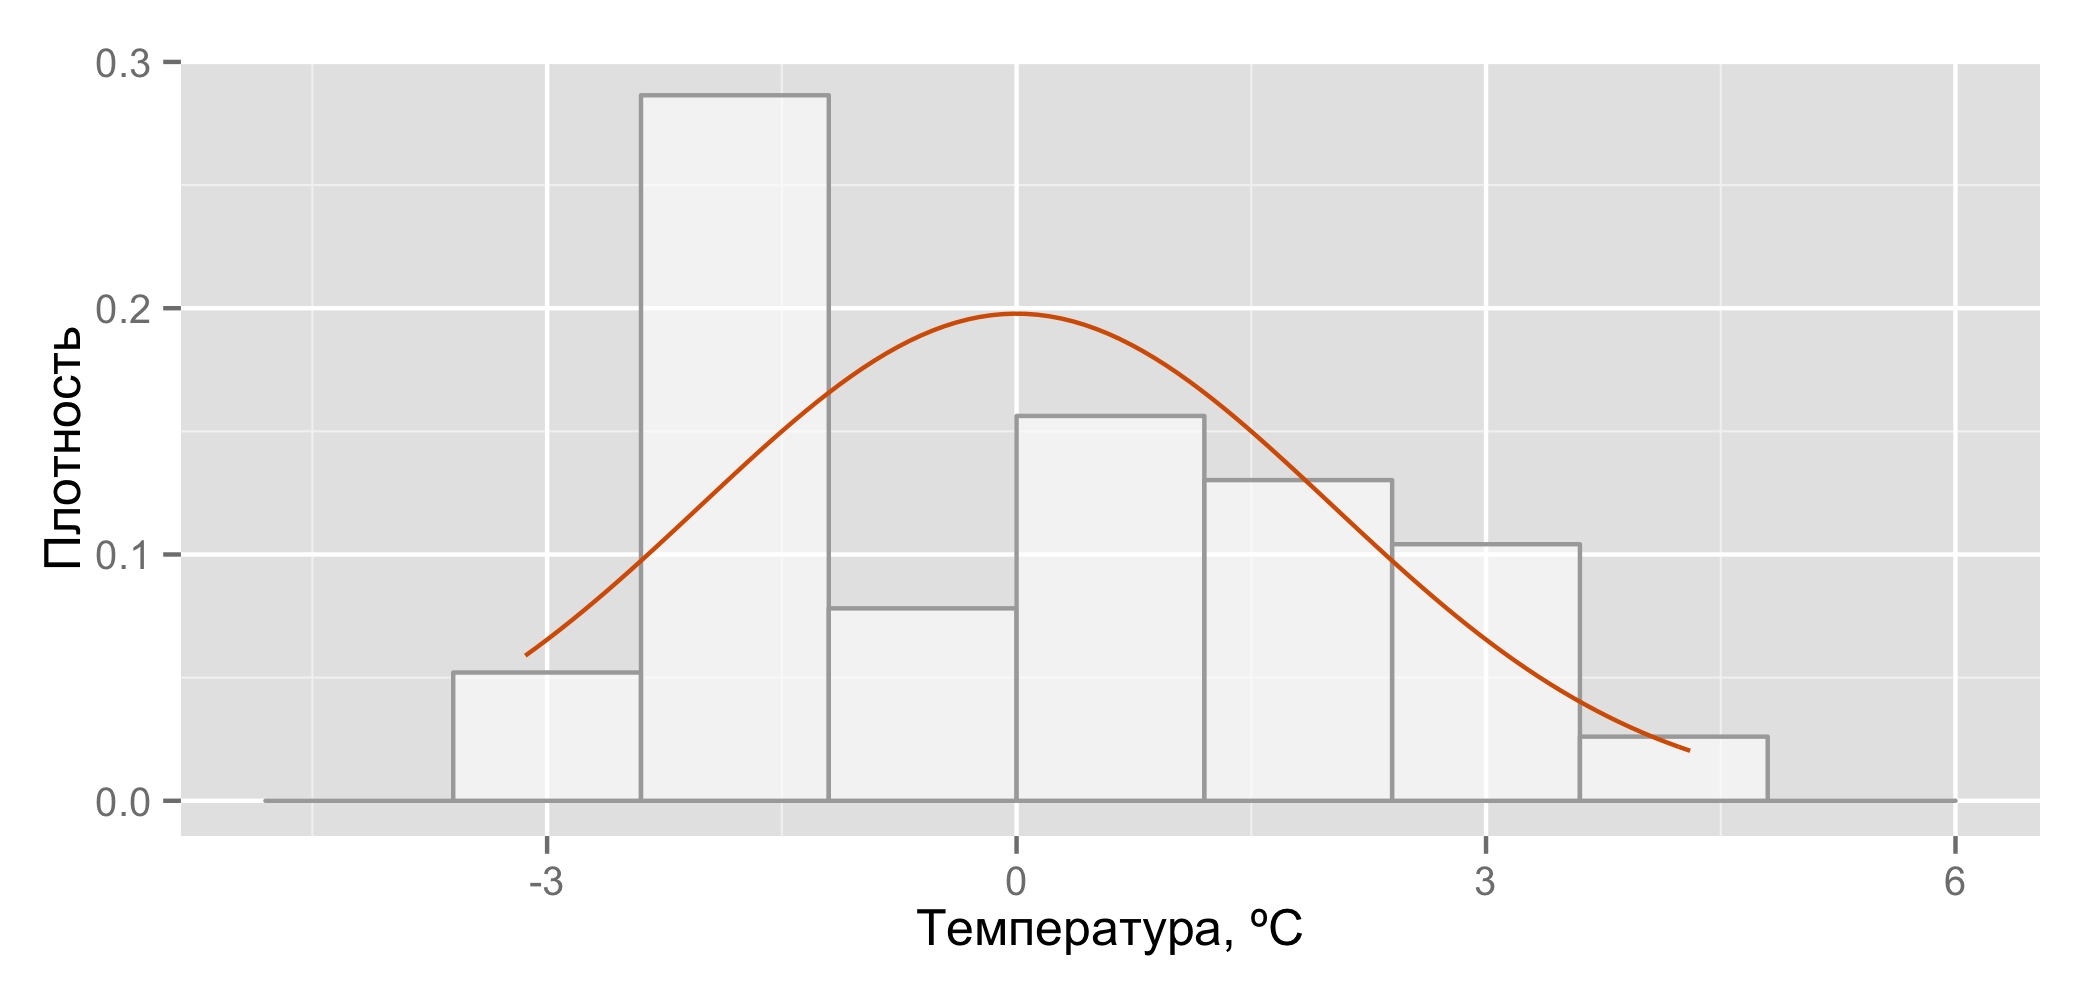
\includegraphics[width=1\linewidth]{../figures/residual/histogram.png}}
\caption{Гистограмма остатков с кривой плотности нормального распределения $\mathcal{N}(19.88, 4.92)$}
\label{img:resid_hist}
\end{figure}

\begin{figure}[H]
	\center{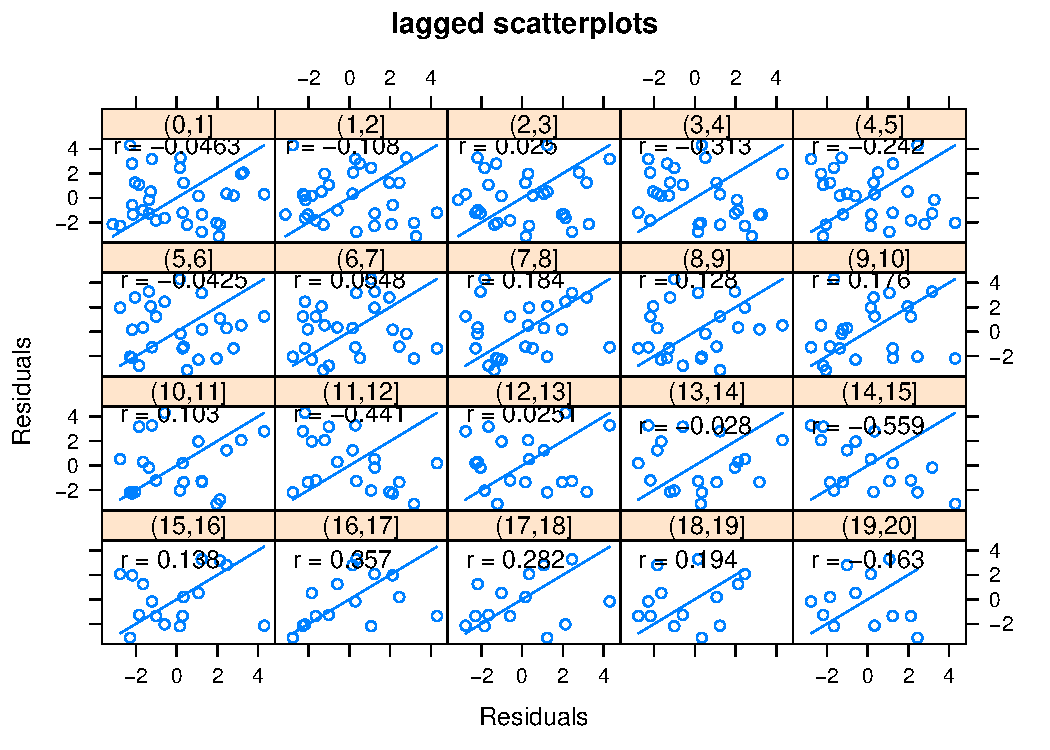
\includegraphics[width=1\linewidth]{../figures/residual/hscat.pdf}}
\caption{Диаграмма взаимного разброса}
\label{img:hscat}
\end{figure}

\begin{figure}[H]
	\center{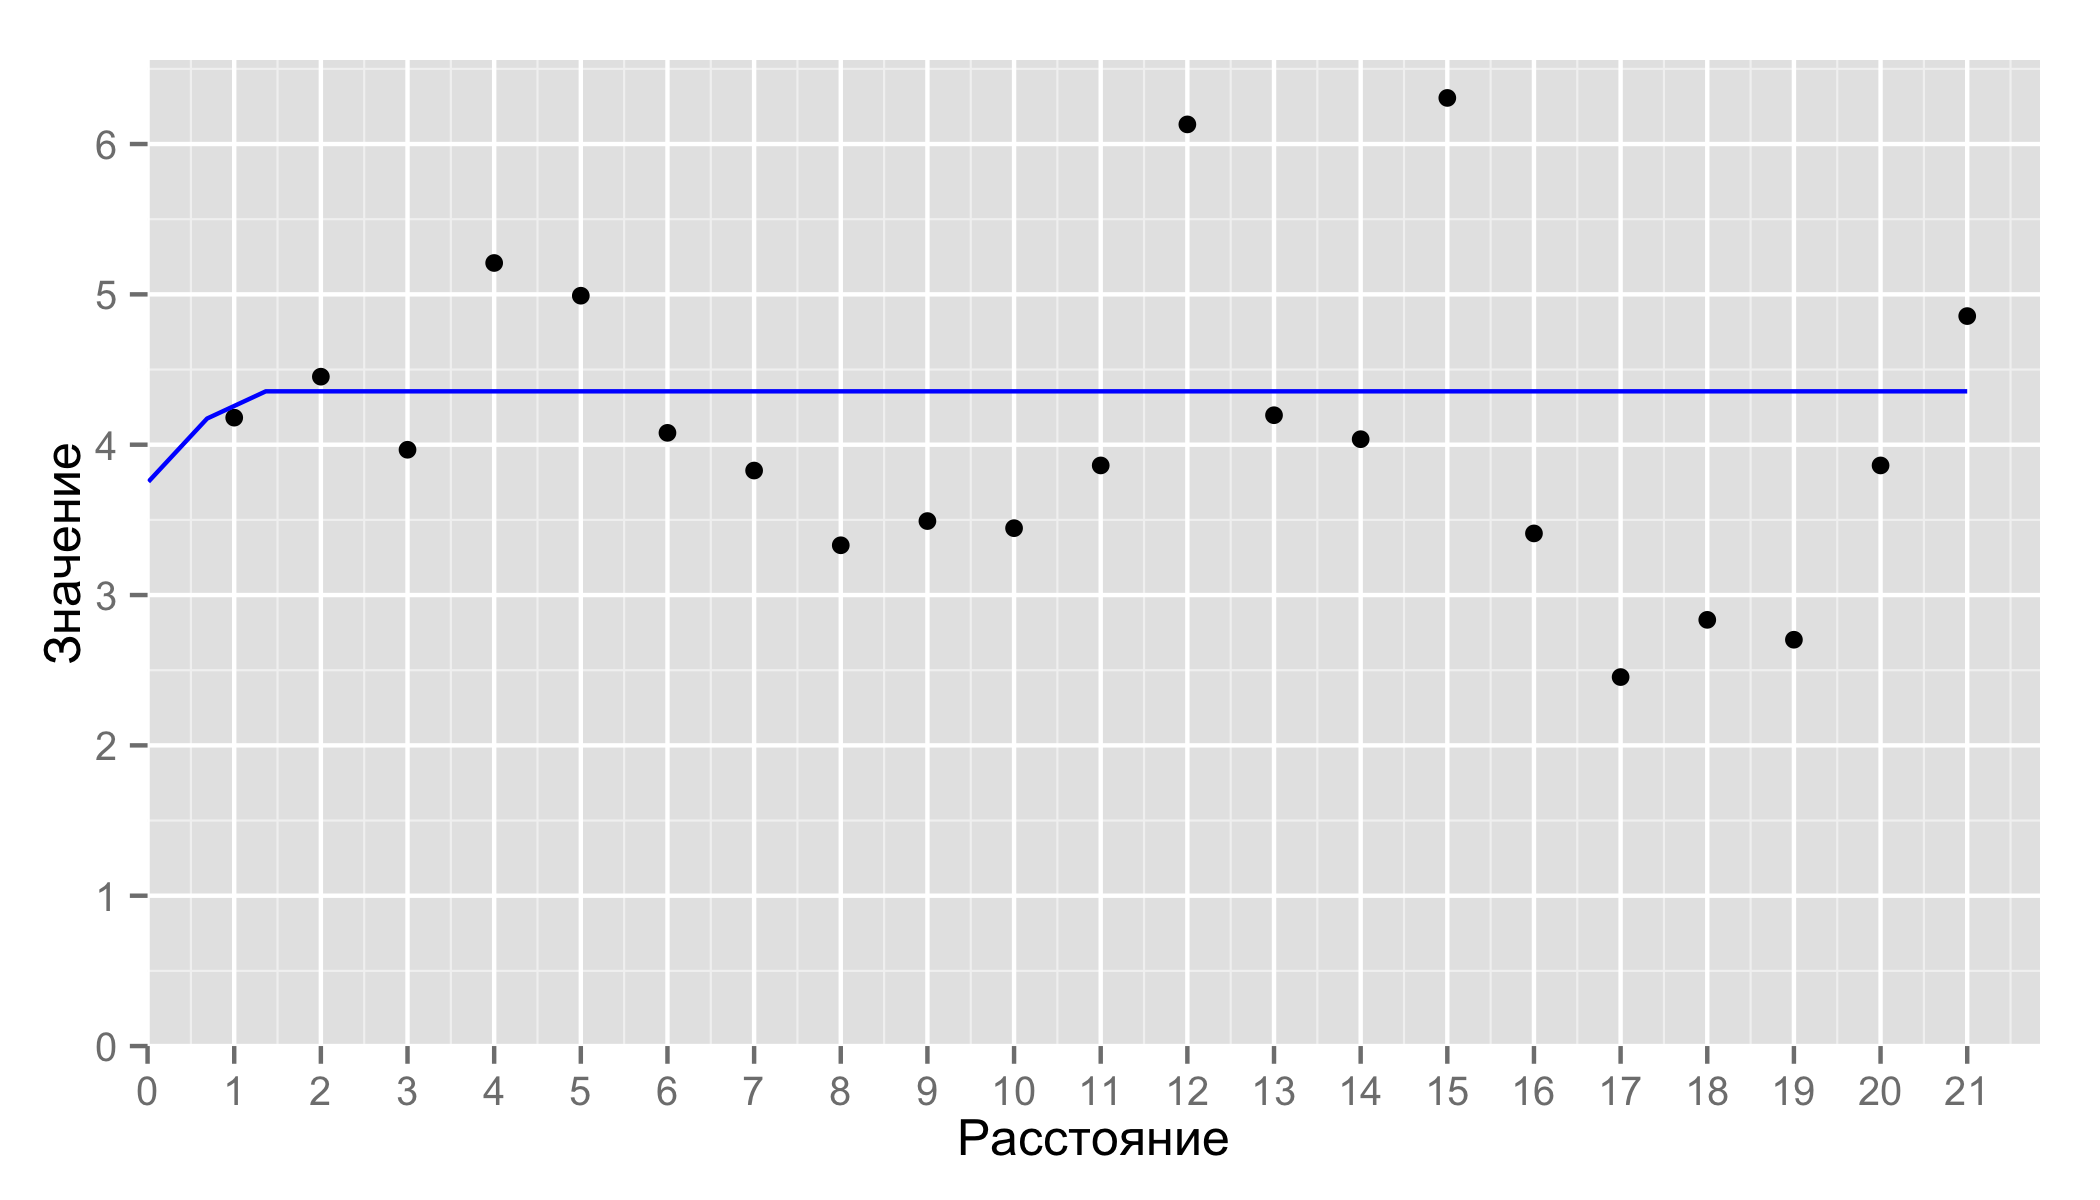
\includegraphics[width=1\linewidth]{../figures/variogram/manual-variogram.png}}
\caption{Экспериментальная и теоретическая вариограмма (сферическая модель)}
\label{img:manual-variogram}
\end{figure}

\begin{figure}[H]
	\center{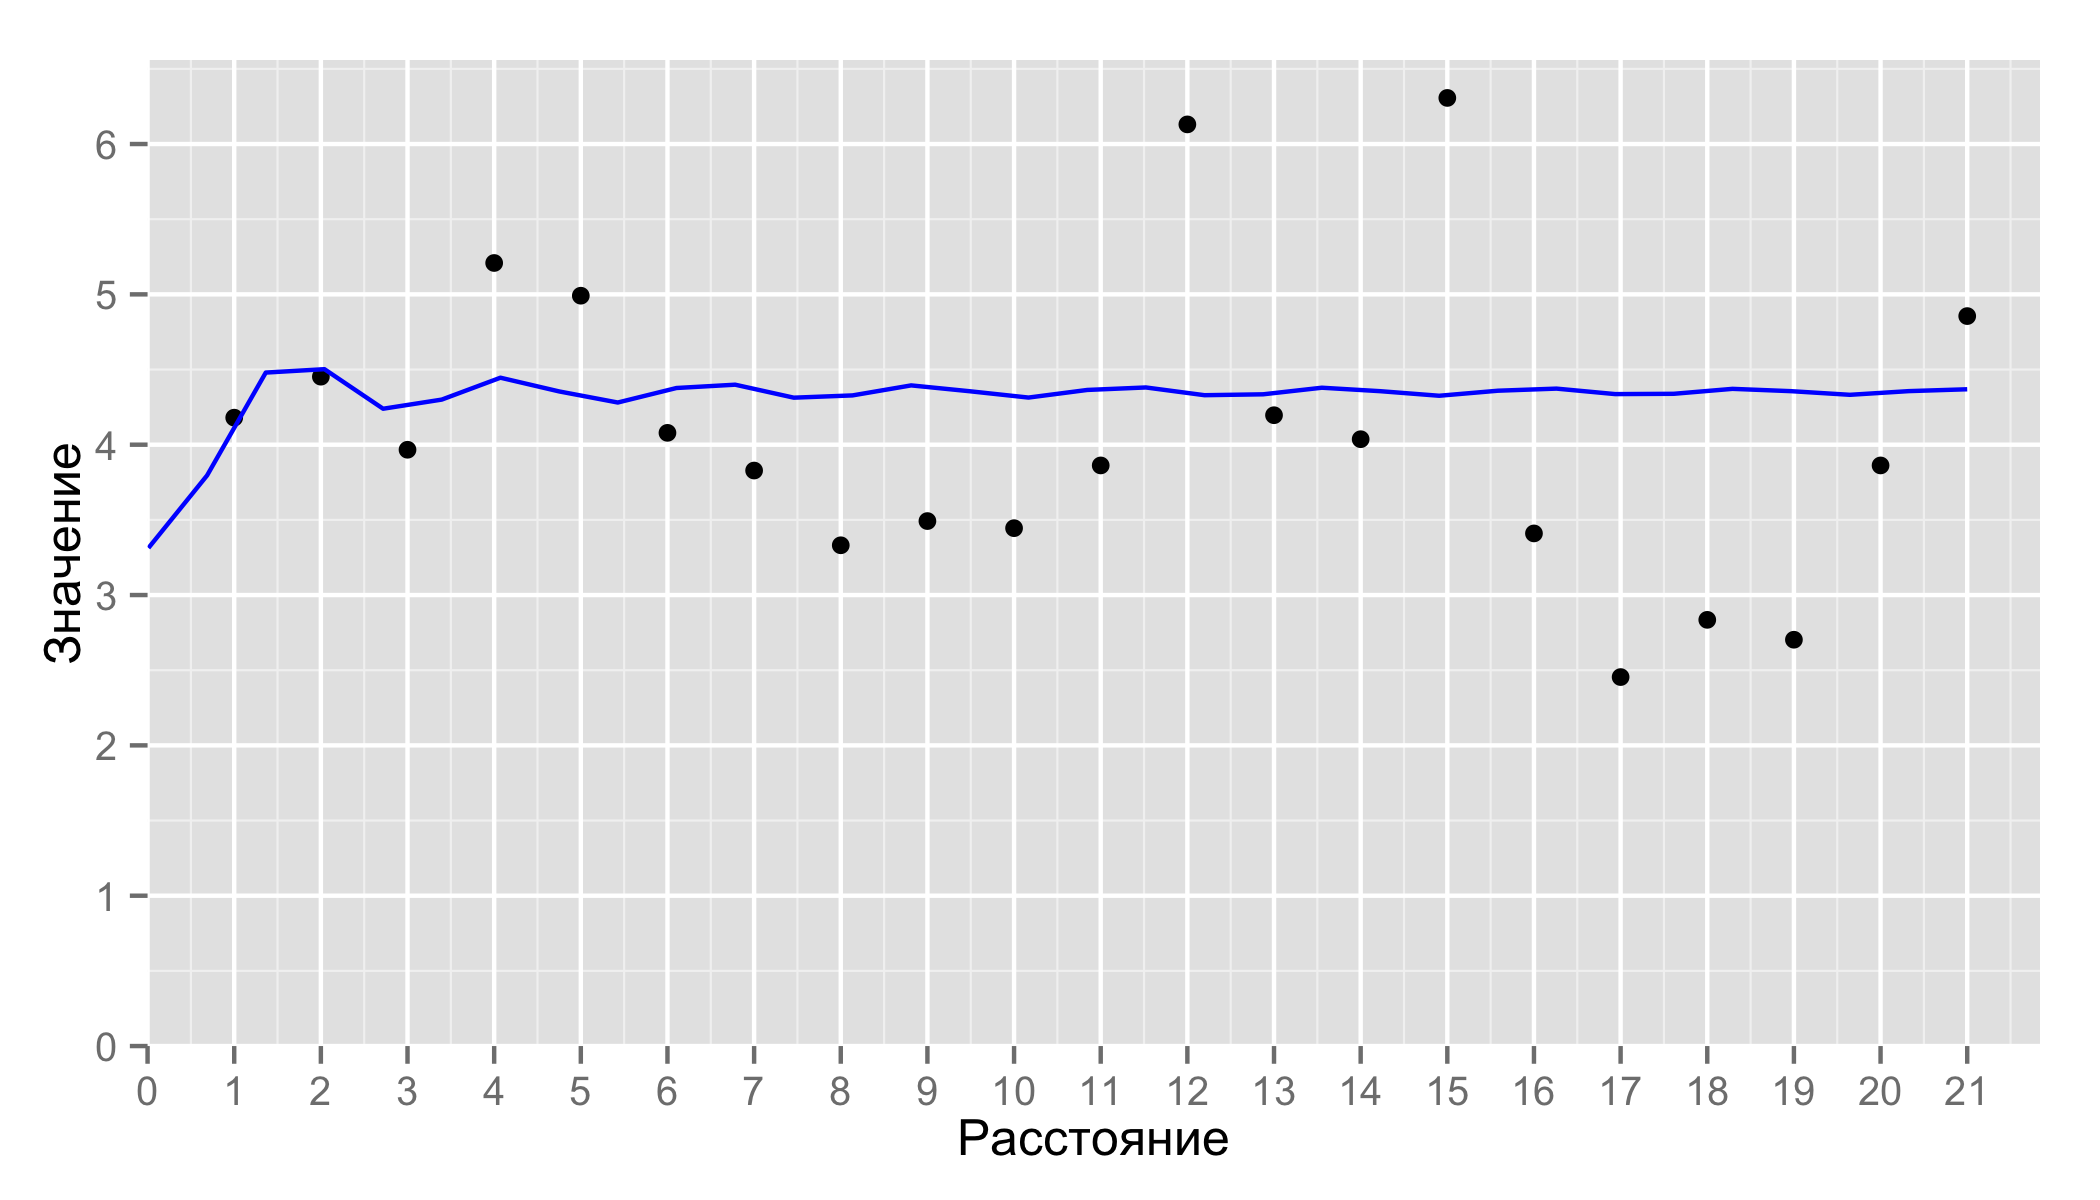
\includegraphics[width=1\linewidth]{../figures/variogram/classical-variogram.png}}
\caption{Экспериментальная и теоретическая вариограмма (классическая оценка)}
\label{img:classical-variogram}
\end{figure}

\begin{figure}[H]
	\center{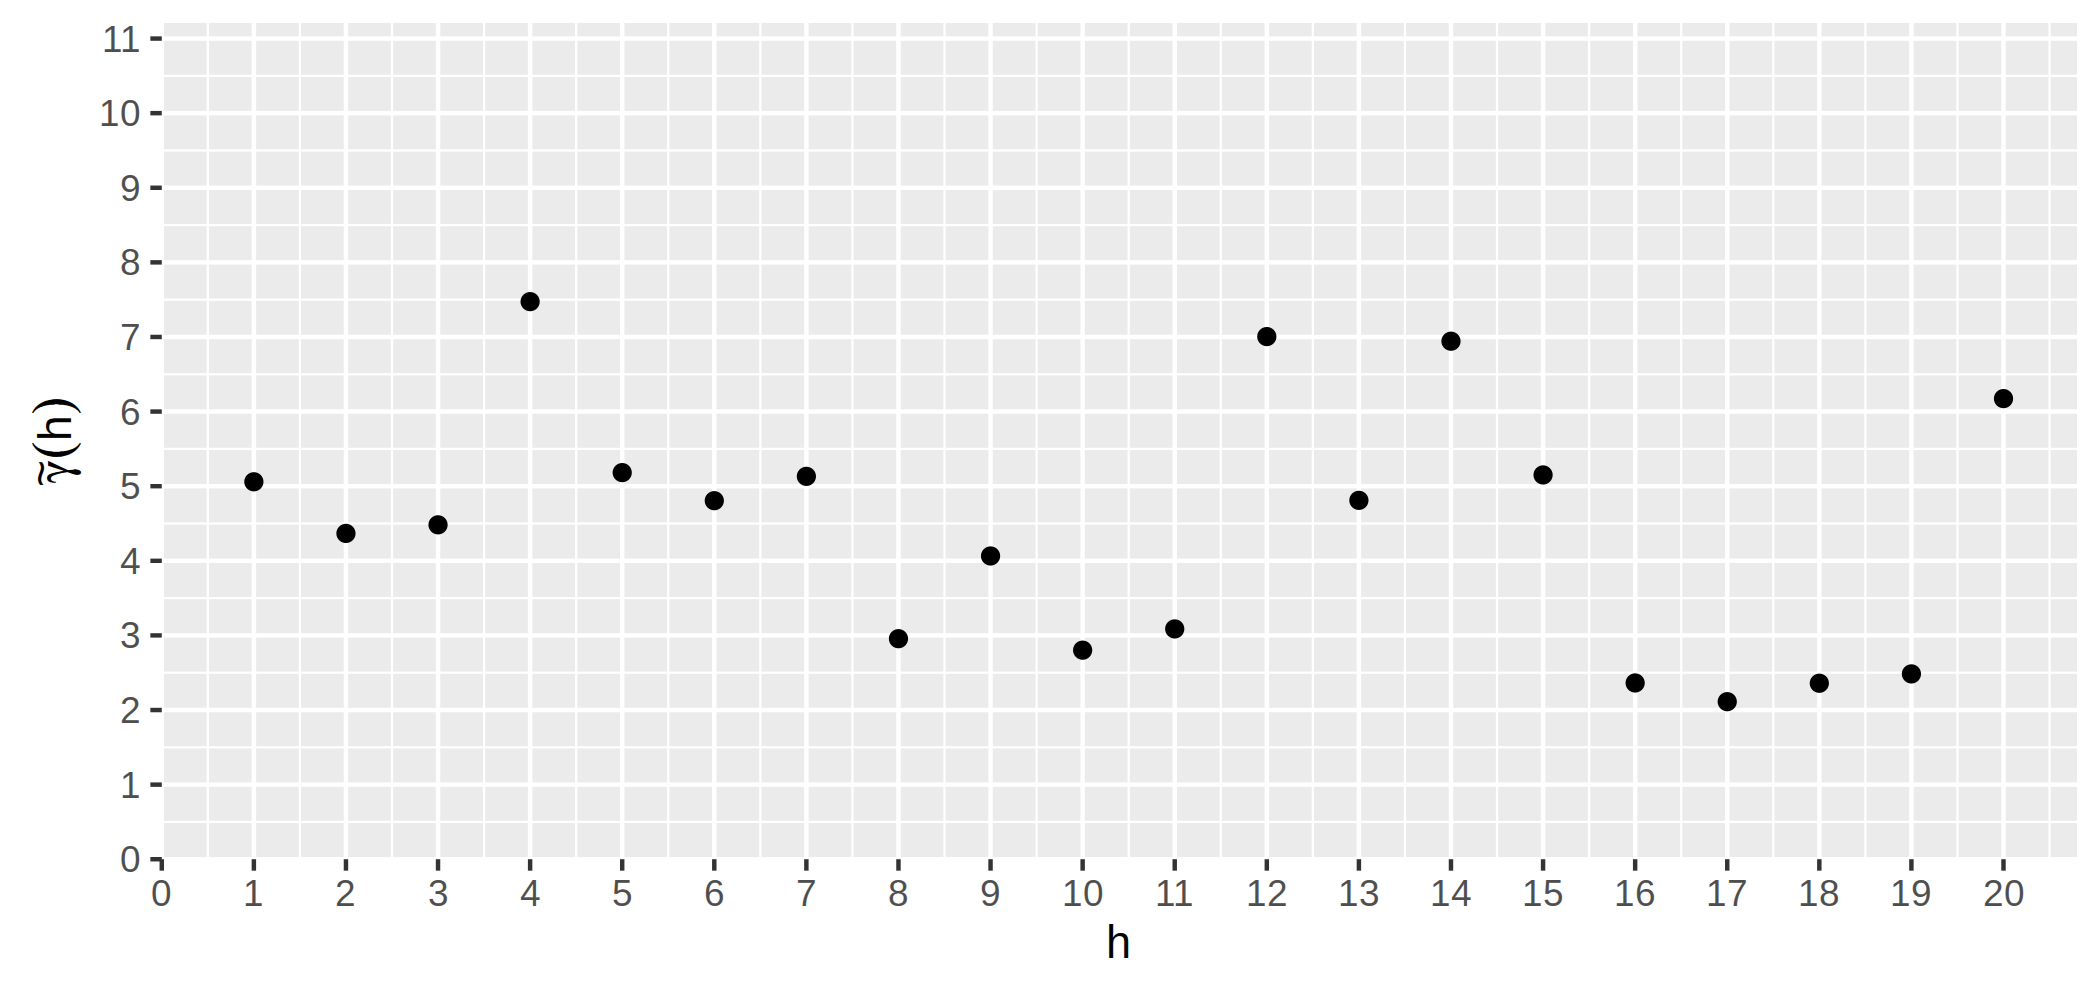
\includegraphics[width=1\linewidth]{../figures/variogram/robust-variogram.png}}
\caption{Экспериментальная и теоретическая вариограмма (робастная оценка)}
\label{img:robust-variogram}
\end{figure}

\begin{figure}[H]
\center{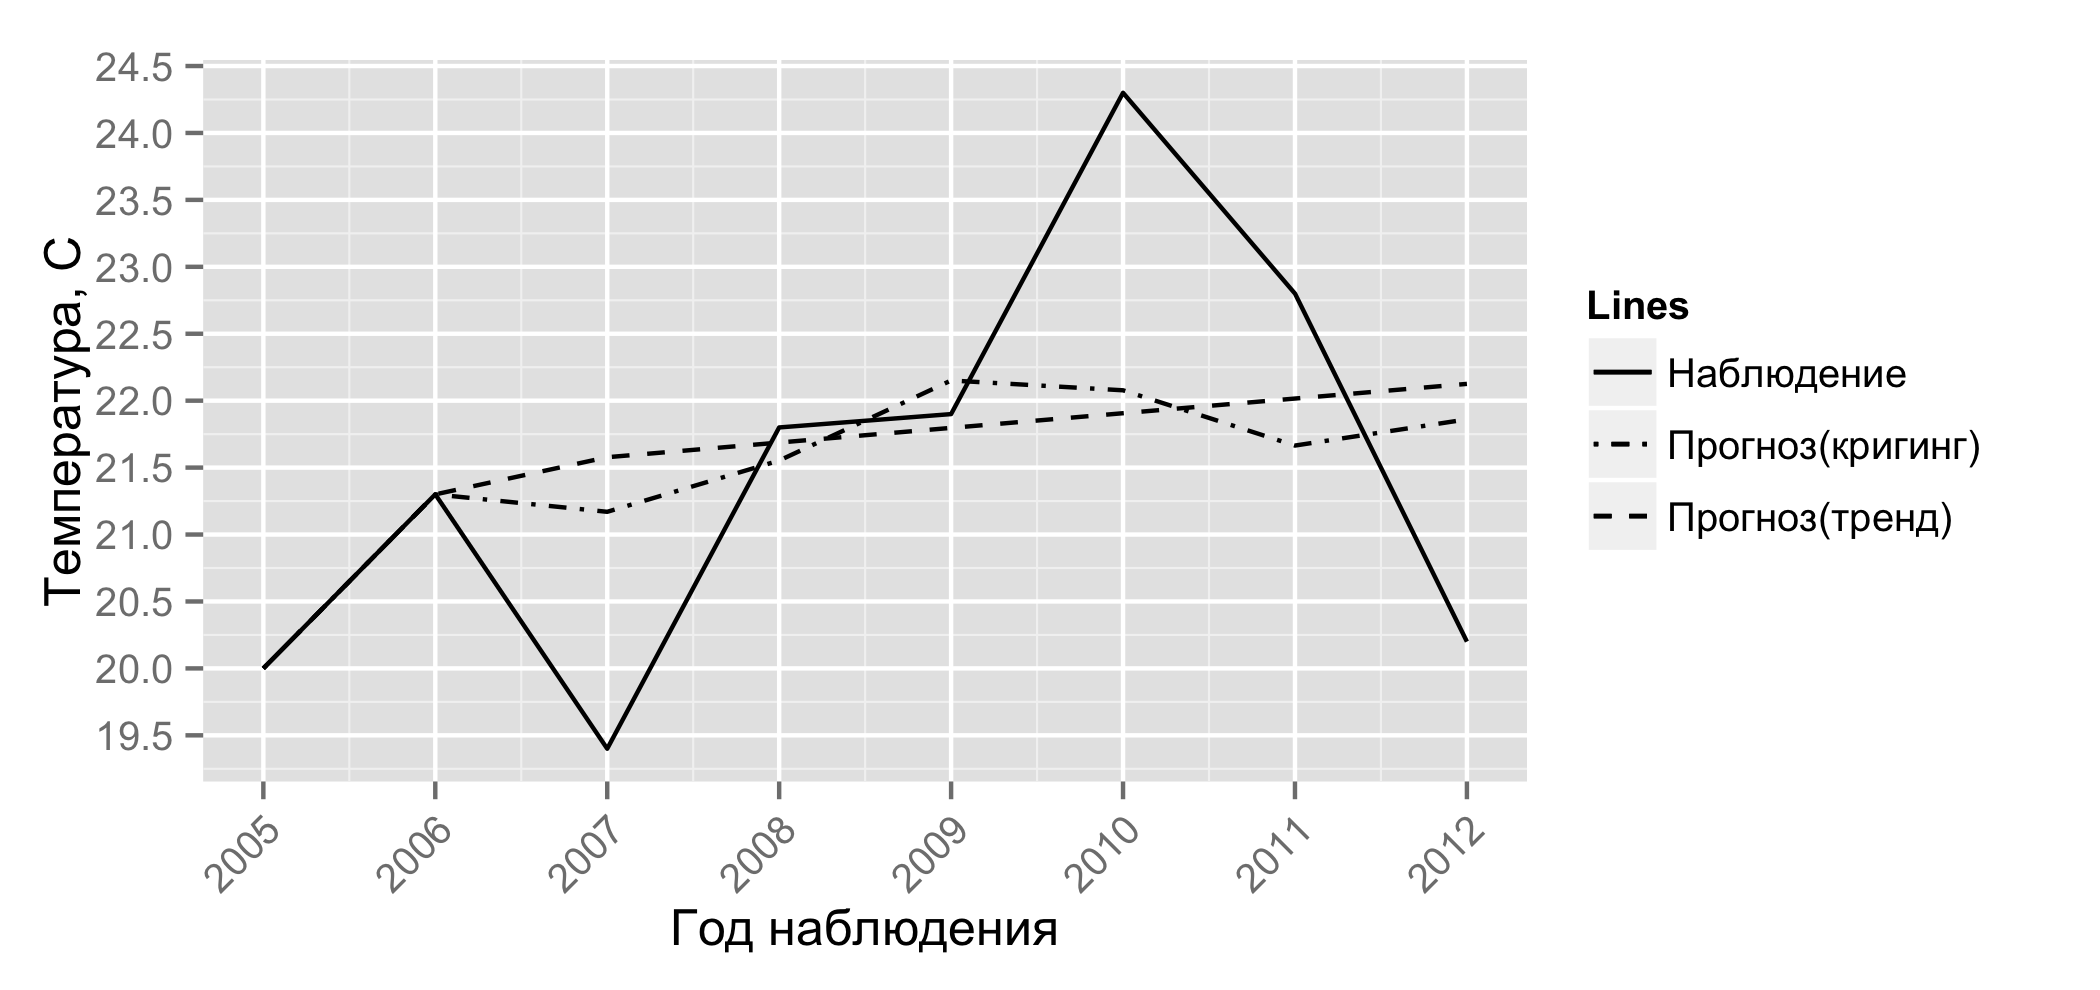
\includegraphics[width=1\linewidth]{../figures/variogram/classical-best-cross-prediction.png}}
\caption{Сравнение прогнозных значений (классическаая оценка)}
\label{img:classical-best-cross-prediction}
\end{figure}

\begin{figure}[H]
\center{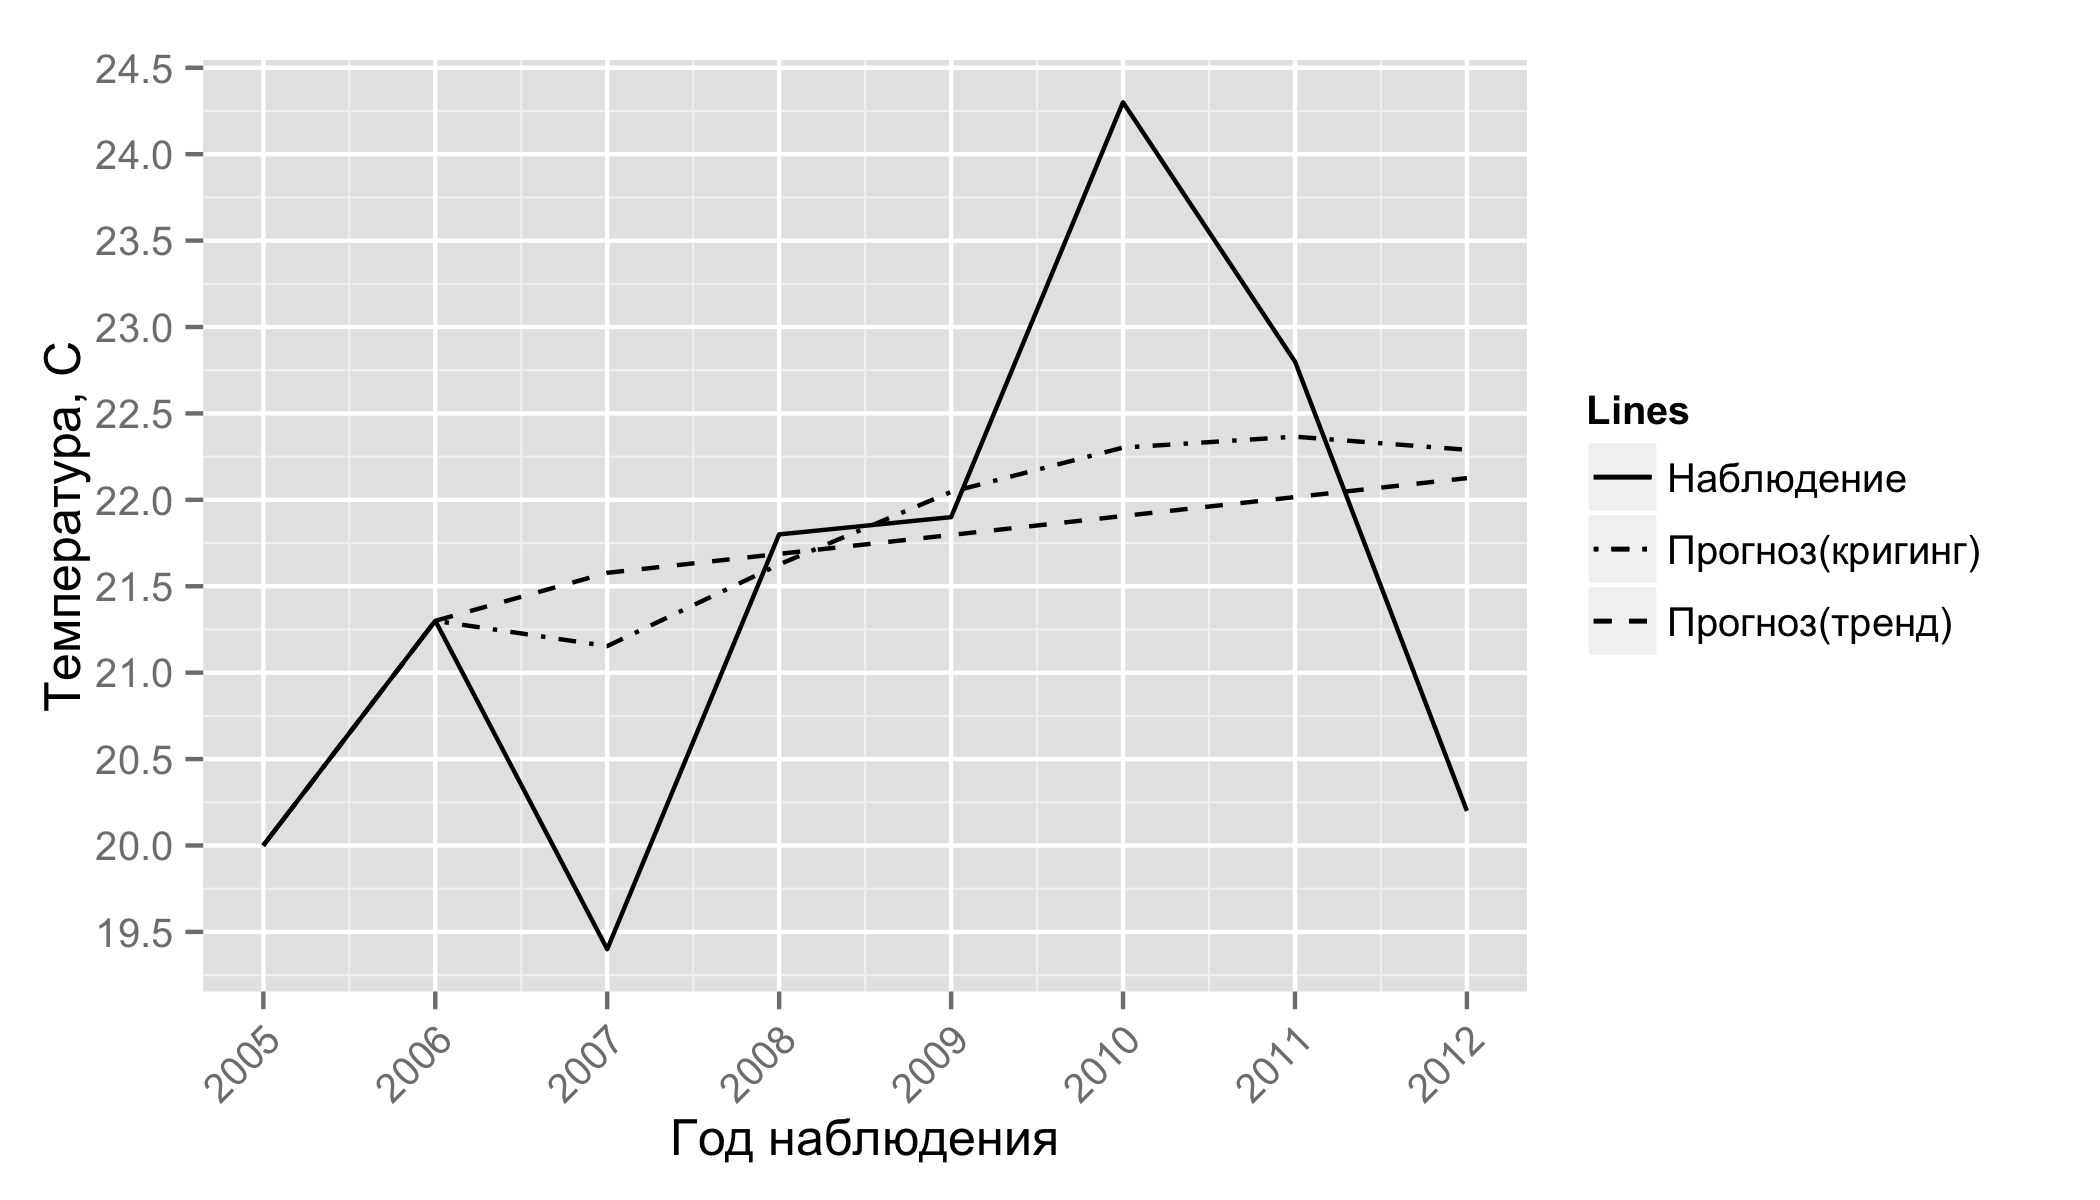
\includegraphics[width=1\linewidth]{../figures/variogram/robust-best-cross-prediction.png}}
\caption{Сравнение прогнозных значений (робастная оценка)}
\label{img:robust-best-cross-prediction}
\end{figure}

\newpage
\section{ Результаты вычислений}
\label{c:app_results}

% latex table generated in R 3.1.2 by xtable 1.7-4 package
% Fri May 15 03:15:00 2015
\begin{table}[H]
\centering
\begin{tabular}{rrr}
  \hline
 & year & temperature \\ 
  \hline
1 & 1975.00 & 2.05 \\ 
  2 & 1976.00 & -2.25 \\ 
  3 & 1977.00 & -0.66 \\ 
  4 & 1978.00 & -1.71 \\ 
  5 & 1979.00 & -1.06 \\ 
  6 & 1980.00 & -1.89 \\ 
  7 & 1981.00 & 1.04 \\ 
  8 & 1982.00 & 0.14 \\ 
  9 & 1983.00 & 2.44 \\ 
  10 & 1984.00 & 0.33 \\ 
  11 & 1985.00 & 1.23 \\ 
  12 & 1986.00 & -2.77 \\ 
  13 & 1987.00 & -2.27 \\ 
  14 & 1988.00 & 4.33 \\ 
  15 & 1989.00 & 0.33 \\ 
  16 & 1990.00 & -1.17 \\ 
  17 & 1991.00 & 3.22 \\ 
  18 & 1992.00 & 2.02 \\ 
  19 & 1993.00 & -1.98 \\ 
  20 & 1994.00 & 1.32 \\ 
  21 & 1995.00 & -1.28 \\ 
  22 & 1996.00 & -1.18 \\ 
  23 & 1997.00 & 0.62 \\ 
  24 & 1998.00 & -2.09 \\ 
  25 & 1999.00 & 2.91 \\ 
  26 & 2000.00 & 0.31 \\ 
  27 & 2001.00 & 3.41 \\ 
  28 & 2002.00 & 2.21 \\ 
  29 & 2003.00 & -2.99 \\ 
  30 & 2004.00 & -1.99 \\ 
  31 & 2005.00 & -1.20 \\ 
  32 & 2006.00 & 0.00 \\ 
  33 & 2007.00 & -2.00 \\ 
  34 & 2008.00 & 0.30 \\ 
  35 & 2009.00 & 0.30 \\ 
   \hline
\end{tabular}
\caption{Временной ряд остатков.} 
\label{table:residuals}
\end{table}

% latex table generated in R 3.1.3 by xtable 1.7-4 package
% Tue May 19 03:07:10 2015
\begin{table}[ht]
\centering
\begin{tabular}{rrrrr}
  \hline
 & Год & Наблюдение & Прогноз & Тренд \\ 
  \hline
1 & 2007 & 19.400 & 21.577 & 21.578 \\ 
  2 & 2008 & 21.800 & 21.688 & 21.687 \\ 
  3 & 2009 & 21.900 & 21.798 & 21.797 \\ 
  4 & 2010 & 24.300 & 21.907 & 21.906 \\ 
  5 & 2011 & 22.800 & 22.017 & 22.016 \\ 
  6 & 2012 & 20.200 & 22.126 & 22.126 \\ 
   \hline
\end{tabular}
\caption{Прогноз (сферическая модель)} 
\label{table:manual-prediction}
\end{table}


\newpage
\section{ Код программ}
\label{c:listings}
\renewcommand{\thelstlisting}{D.1}
\lstinputlisting[language=R, caption=Описательные статистики, label=lst:dstats]{../R/lib/dstats.R}
\renewcommand{\thelstlisting}{D.2}
\lstinputlisting[language=R, caption=Основной код программы, label=lst:main]{../R/master.R}
\renewcommand{\thelstlisting}{D.3}
\lstinputlisting[language=R, caption=Вариограммный анализ, label=lst:variogram]{../R/predictor.R}